% Symmetry-constrained spectral fibres: reverse-complement group actions on double-stranded DNA and the
% fibres of circular molecular fingerprints
% Build (in this folder): pdflatex symmetry_fibres (x2)
\documentclass[11pt]{article}
\usepackage{lmodern}
\usepackage[T1]{fontenc}
\usepackage{amsmath,amssymb,amsthm,mathtools}
\usepackage[margin=1.05in]{geometry}
\usepackage{booktabs,array}
\usepackage{microtype}
\usepackage{xcolor}
\usepackage{tikz}
\usetikzlibrary{arrows.meta,positioning}
\usepackage[hidelinks]{hyperref}
\newcommand{\doi}[1]{\href{https://doi.org/#1}{\nolinkurl{doi:#1}}}
\emergencystretch=2em

\theoremstyle{plain}
\newtheorem{theorem}{Theorem}
\newtheorem{proposition}[theorem]{Proposition}
\newtheorem{lemma}[theorem]{Lemma}
\newtheorem{corollary}[theorem]{Corollary}
\theoremstyle{definition}
\newtheorem{definition}[theorem]{Definition}
\newtheorem{example}[theorem]{Example}
\theoremstyle{remark}
\newtheorem{remark}[theorem]{Remark}

\newcommand{\spec}{\operatorname{spec}}
\newcommand{\DS}{\mathrm{DS}}
\newcommand{\env}{\operatorname{env}}
\newcommand{\Fib}{\mathcal F}

\title{\bfseries Symmetry-constrained spectral fibres:\\ reverse-complement group actions on double-stranded
DNA\\ and the fibres of circular molecular fingerprints}
\author{Zhengyi Chen\\[2pt]
\normalsize\begin{tabular}{c}
Guangxi Key Laboratory of Drug Discovery and Optimization,\\
Guangxi Engineering Research Center for Pharmaceutical Molecular Screening\\
and Druggability Evaluation, School of Pharmacy, Guilin Medical University,\\
Guilin 541199, P.~R.~China\\
\texttt{chenzhengyi@glmc.edu.cn}
\end{tabular}
\and
Ruqing Chen\\[2pt]
\normalsize GUT Geoservice Inc., Montreal, Qu\'ebec, Canada\\
\normalsize\texttt{ruqing@hotmail.com}}
\date{27 September 2026\\[4pt]\small DOI: \href{https://doi.org/10.5281/zenodo.23002923}{10.5281/zenodo.23002923}}

\begin{document}
\maketitle

\begin{abstract}
\noindent
A representation that depends on an object only through its local content is constant on the
\emph{spectral fibre} of the object, the set of objects with the same multiset of local pieces. For
protein sequences the pieces are $k$-mers and the fibres are Eulerian trails of a de~Bruijn graph. This
paper treats two settings in which a symmetry enters. For double-stranded DNA the group $G=\{e,\rho\}$
generated by reverse complementation acts on sequence space, a strand-agnostic encoder is $G$-invariant,
and its fibre is the set $\DS(S,k)$ of sequences with the same double-stranded spectrum. This fibre is not a
single Eulerian count: it is a sum of BEST determinants over the points of a lattice, the $(-1)$-eigenlattice
of $\rho$ on the circulations of a double cover, and counting it is $\#$P-hard. For bacteriophage
$\phi$X174 at $k=10$, $|\DS|=31\,925\,753\,246\,212$, between the single-strand count $8\,610\,708\,632$ and
the $1.4\cdot10^{36}$ Eulerian circuits of the double cover, which is what a naive count would give. For small
molecules the local pieces are the atom environments of circular fingerprints, and the symmetry is built into
their construction, because the neighbours of an atom are unordered. We prove that on substituted linear
chains the radius-$r$ Morgan (ECFP$_{2r}$) partition is exactly the spectrum of $(2r+1)$-windows read up to
reversal, with the substituent at distance $r$ coarsened to its atom type, and confirm this by exhaustive
enumeration of $19\,683$ chains. We construct distinct molecules with identical ECFP4 and ECFP6 fingerprints
(2048-bit, count and unhashed) in which the topological distance between two pharmacophoric groups changes from
$7$ to $12$ bonds, and we measure that $3.2\%$ of the $9\,963$ chains with nine substituted positions share
their ECFP4 with another molecule. A common quotient framework covers composition encoders, convolutional
encoders, strand-agnostic DNA encoders and circular fingerprints.
\end{abstract}

\medskip
\noindent\textbf{Keywords.} reverse complement, double-stranded DNA, de~Bruijn graph, BEST theorem, lattice
sum, $\phi$X174, extended-connectivity fingerprint, Morgan algorithm, Weisfeiler--Lehman, quotient space,
group action.

% ================================================================ 1
\section{Introduction}\label{sec:intro}

A \emph{local} representation of a discrete object depends on it only through the multiset of its local
pieces. For a sequence the pieces are the $k$-mers; for a molecular graph they are the atom environments of
radius $r$. Two objects with the same multiset receive the same representation, whatever the representation
was trained to do. We called the set of such objects the spectral fibre of an object, computed its size exactly
for every human protein, and showed which encoder architectures are confined to it
\cite{CC26a,CC26b,CC26c,CC26d}.

Those papers concern one strand of a linear sequence. Two settings that matter in practice carry a symmetry
in addition. A regulatory element or a CRISPR target has no preferred strand, so a DNA encoder should give the
same output to a sequence and its reverse complement. A molecule has no preferred orientation, and the
environments that circular fingerprints hash are unordered. In both cases the fibre of the representation is
larger than the one-strand fibre, and in the DNA case it is also much harder to count. The combinatorics of
the double-stranded fibre is developed in the monograph \cite{AG}: the lattice-sum formula, the $\#$P-hardness,
the moves that connect the fibre, and the computation for $\phi$X174. The present paper does not add to that
combinatorics. Its contributions are the following.
\begin{enumerate}
\item A formulation of both settings as quotients of an object space by a group action followed by a local
statistic (Sections~\ref{sec:dna} and~\ref{sec:unified}), which makes precise why a strand-agnostic encoder is
blind to the double-stranded fibre and not only to the one-strand fibre.
\item An account of the $\phi$X174 numbers in this light (Section~\ref{sec:phix}), including the comparison
between the true fibre, the one-strand fibres and the Eulerian circuits of the double cover, which differ by
$26$ orders of magnitude.
\item An exact description of the fibres of Morgan fingerprints on substituted linear chains
(Theorem~\ref{thm:chain}), verified exhaustively; explicit collision pairs at ECFP4 and ECFP6 with changed
pharmacophore geometry; and a census of collisions (Section~\ref{sec:ecfp}).
\end{enumerate}

% ================================================================ 2
\section{Double-stranded DNA as a group quotient}\label{sec:dna}

Let $\Sigma=\{\mathtt A,\mathtt C,\mathtt G,\mathtt T\}$ and let $\rho$ be reverse complementation,
$\rho(S)=\overline{S}$. It is an involution on $\Sigma^L$ and on circular sequences, so $G=\{e,\rho\}\cong\mathbb Z/2$
acts on sequence space. A \emph{strand-agnostic} encoder is a $G$-invariant map $\phi$, i.e.\ $\phi(S)=\phi(\rho S)$.
It factors through the orbit space $\Sigma^L/G$.

\begin{definition}[double-stranded spectrum]\label{def:dsspec}
The \emph{double-stranded $k$-spectrum} of $S$ is the multiset $\spec_k(S)+\spec_k(\rho S)$. For circular $S$, the
\emph{double-stranded fibre} is
\[
\DS(S,k)=\{T\ \text{circular}:\ \spec_{k+1}(T)+\spec_{k+1}(\rho T)=\spec_{k+1}(S)+\spec_{k+1}(\rho S)\},
\]
counted with $T$ and $\rho T$ as distinct elements unless equal \cite[Def.~7.3]{AG}. The index convention follows
\cite{AG}: $\DS(S,k)$ is defined by $(k+1)$-mers, the $k$-mers being the vertices of the graph below.
\end{definition}

\begin{proposition}[what a strand-agnostic local encoder sees]\label{prop:dslocal}
Let $\phi$ be local of order $k+1$ on circular sequences, i.e.\ $\phi(T)$ depends on $T$ only through
$\spec_{k+1}(T)$, and $G$-invariant. Then $\phi$ is constant on $\DS(S,k)$, and $\DS(S,k)\supseteq F_{k+1}(S)\cup F_{k+1}(\rho S)$.
\end{proposition}

\begin{proof}
For $T\in\DS(S,k)$ the two strands of $T$ together have the same $(k+1)$-mers as the two strands of $S$. A
$G$-invariant $\phi$ may be written as $\phi(T)=\psi(\spec_{k+1}(T)+\spec_{k+1}(\rho T))$: indeed
$\phi(T)=\tfrac12(\phi(T)+\phi(\rho T))$ and each summand is a function of one strand's spectrum, but the pair of
spectra is determined only up to order by the sum; since $\phi(T)=\phi(\rho T)$, the value does not depend on which
of the two spectra is called the first. The inclusion holds because $T\in F_{k+1}(S)$ gives $\spec_{k+1}(T)=\spec_{k+1}(S)$
and then $\spec_{k+1}(\rho T)=\spec_{k+1}(\rho S)$, the spectrum of the reverse complement being determined by that of
the sequence.
\end{proof}

So the price of strand invariance is exact. A one-strand local encoder is blind to $F_{k+1}(S)$; a strand-agnostic
one is blind to $\DS(S,k)$, which contains the one-strand fibres of both strands and, in general, much more.

\paragraph{The double cover and the lattice.} Let $D_k$ be the de~Bruijn multigraph on the $k$-mers of $S$ and
of $\rho S$ together, with one arc per $(k+1)$-mer occurrence on either strand. Reverse complementation acts on
$D_k$ as a fixed-point-free involution $\rho$ of the arcs that reverses direction \cite[Ch.~5--6]{AG}. A
circular sequence $T$ with the double-stranded spectrum of $S$ corresponds to a pair of Eulerian circuits, one
through each strand, whose arc-usage vectors $c$ and $\rho c$ add up to the multiplicity vector $m$ of $D_k$. The
usage $c$ is a circulation of $D_k$, and $c+\rho c=m$ says that $f=c-\rho c$ lies in the $(-1)$-eigenlattice
$\Lambda^-$ of $\rho$ on the circulation lattice, inside the box $|f|\le m$ with $f\equiv m\bmod2$.

\begin{theorem}[the fibre is a lattice sum {\cite[Thm.~7.6]{AG}}]\label{thm:lattice}
\[
|\DS(S,k)|=\sum_{f\in\Lambda^-\cap\{|f|\le m,\ f\equiv m\ (2)\}}N_{\mathrm{seq}}\Bigl(\tfrac{m+f}{2}\Bigr),
\]
where $N_{\mathrm{seq}}(c)$ is the number of circular sequences that use each arc exactly $c(a)$ times, which is
$0$ unless the support of $c$ is connected and otherwise $t(G_c)\operatorname{Loc}(G_c)/\prod_ac(a)!$ by the BEST
theorem \cite{BEST}. The rank of $\Lambda^-$ is $(|A|-|V|+2-\#\mathrm{fix}_A-\#\mathrm{fix}_V)/2$, the Hopf trace of
$\rho$ \cite[Ch.~7, check~L]{AG}.
\end{theorem}

Two consequences separate this fibre from the one-strand case. First, there is no single determinant: the
sum runs over a lattice whose rank grows with the number of shared $k$-mers between the strands, and
evaluating it is $\#$P-hard in general \cite[Cor.~10.6]{AG}. Second, the Eulerian circuits of $D_k$ itself do not
count the fibre. A circuit of $D_k$ walks through both strands as one closed walk; it corresponds to a
double-stranded reconstruction only when its usage vector is of the form $c$ with $c+\rho c=m$, and each
reconstruction is then counted with the multiplicity $\prod c(a)!$ and once per rotation. The BEST count of
$D_k$ is therefore an upper bound that is astronomically loose (Section~\ref{sec:phix}).

\paragraph{Moves.} On one strand, fibre members differ by transpositions of segments between repeated
$k$-mers \cite{Ukk92,Pev95}. On two strands there is a second move: a segment flanked by an inverted repeat
$w\cdots\rho w$ may be replaced by its reverse complement without changing the double-stranded spectrum
\cite[Thm.~11.1]{AG} (Figure~\ref{fig:moves}a). Transpositions between direct repeats and inversions between inverted repeats are the two
products of non-allelic homologous recombination, so a strand-agnostic local encoder is blind to exactly the
rearrangements that recombination between repeats of length $k$ produces. Whether the two moves together with
$\rho$ connect every double-stranded fibre is conjectured, and proved for the palindromic genomes of
\cite[Ch.~10--11]{AG}.

% ================================================================ 3
\section{The reconstruction ambiguity of \texorpdfstring{$\phi$}{phi}X174}\label{sec:phix}

Bacteriophage $\phi$X174 (RefSeq NC\_001422.1) is a circular single-stranded DNA genome of $5\,386$ bp whose
replicative form is double-stranded. Table~\ref{tab:phix} collects the numbers computed in \cite{AG} from the
lattice sum, by three independent algorithms at $k=11$ and $12$ (brute force, a fermionic frontier sweep and an
arborescence frontier) and by a compiled enumeration of the half-box at $k=10$, whose $1\,240\,843\,950$ points
were processed modulo five primes and recombined by the Chinese remainder theorem
\cite[Ch.~8--9]{AG}.

\begin{table}[t]
\centering\small
\begin{tabular}{rrrrrrr}
\toprule
$k$ & rank $\Lambda^-$ & box points & connected & $|\DS(S,k)|$ & $N_{\mathrm{seq}}(S)+N_{\mathrm{seq}}(\rho S)$ & $\mathrm{ec}(D_k)$\\
\midrule
12 & 4 & 10 & 8 & 10 & 4 & 33\\
11 & 12 & 528 & 218 & 864 & 66 & 25\,318\,912\\
10 & 48 & 2\,481\,687\,900 & 909\,103\,210 & 31\,925\,753\,246\,212 & 8\,610\,708\,632 & $1.368\cdot10^{36}$\\
\bottomrule
\end{tabular}
\caption{Double-stranded fibres of $\phi$X174 \cite[Tables of Ch.~7--9]{AG}. Columns: rank of the
$(-1)$-eigenlattice; lattice points in the box; points with connected support; the fibre; the sum of the
one-strand fibres of the two strands; Eulerian circuits of the double cover.}\label{tab:phix}
\end{table}

Three readings of the table. At $k=12$ the two strands share one inverted-repeat pair and one palindrome
(\texttt{TGGAGGCCTCCA}), the lattice has rank $4$, and the fibre has $10$ members against $4$ for the two
one-strand fibres. At $k=10$ the fibre has $3.19\cdot10^{13}$ members. A strand-agnostic local encoder of order
$11$ assigns all of them one vector; a one-strand encoder of the same order is blind to $8.6\cdot10^9$ of them. The
gap is the price of strand invariance for this genome. Finally, the double cover has $1.37\cdot10^{36}$ Eulerian
circuits at $k=10$. Anyone who counted the fibre by applying the BEST theorem to the double cover would
overestimate it by a factor of $4\cdot10^{22}$. The overcount comes from circuits whose usage is not of the form
$c+\rho c=m$ and from the labelling of parallel arcs.

The fibre is connected by the two moves of Section~\ref{sec:dna}: at $k=11$ all $864$ reconstructions and at
$k=12$ all $10$ are reached from $S$ by inversion flips alone, in at most $8$ and $3$ flips
\cite[Ch.~7, \texttt{ds\_flips}]{AG}. The reconstructions are not exotic: each is $\phi$X174 with some segments
between inverted repeats reversed, exactly the sequences that an inversion event would produce.

% ================================================================ 4
\section{Fibres of circular molecular fingerprints}\label{sec:ecfp}

\subsection{Morgan identifiers as a symmetric local statistic}

Extended-connectivity fingerprints \cite{RH10} assign to each atom an identifier of its radius-$r$ environment by
$r$ rounds of the Morgan algorithm \cite{Morgan65}: the identifier of an atom at round $i$ is a hash of its
identifier at round $i-1$ and the unordered multiset of (bond type, neighbour identifier at round $i-1$). This is
Weisfeiler--Lehman colour refinement \cite{WL68,GIN}. The fingerprint is the multiset of identifiers of all atoms at
all rounds $0,\dots,r$, with environments that cover an atom set already covered removed, hashed to a bit vector
(ECFP$_{2r}$) or kept as counts. A molecular encoder built on ECFP is therefore local in the graph sense, and its
fibre is the set of molecules with the same multiset of environments. The symmetry is intrinsic: because the
neighbours are unordered, an environment is read up to the automorphisms that fix its centre.

\subsection{Substituted chains: an exact description}

Consider the molecules $\mathrm{CH_3}$-$(\mathrm{CHR}_1)$-$\cdots$-$(\mathrm{CHR}_N)$-$\mathrm{CH_3}$ with
$R_i\in\{\mathrm H,\mathrm F,\mathrm{Cl}\}$. Each is a string over the alphabet $\{\mathtt H,\mathtt F,\mathtt L\}$
(for $\mathrm{CH_2}$, $\mathrm{CHF}$, $\mathrm{CHCl}$), bounded by terminal methyls $\mathtt M$, and two strings give
the same molecule if and only if they are equal or mirror images. For a letter $x$ let $\bar x$ be its \emph{atom
type}: $\bar{\mathtt F}=\bar{\mathtt L}=\mathtt X$ (a carbon of degree $3$ with one hydrogen), and
$\bar{\mathtt H}=\mathtt H$, $\bar{\mathtt M}=\mathtt M$.

\begin{definition}[coarsened symmetric window spectrum]\label{def:window}
For the chain string $s=\mathtt M s_1\cdots s_N\mathtt M$ and $r\ge1$, the radius-$r$ window of position $i$ is
$w_r(i)=(\bar s_{i-r},s_{i-r+1},\dots,s_{i+r-1},\bar s_{i+r})$, with the symbol $\wedge$ for positions outside the
chain. The \emph{symmetric window spectrum} $\Omega_r(s)$ is the multiset of the classes $\{w_r(i),w_r(i)^{\mathrm{rev}}\}$
over all positions $i$.
\end{definition}

\begin{theorem}[fibres of Morgan fingerprints on chains]\label{thm:chain}
Two chain molecules have the same unhashed radius-$r$ Morgan count fingerprint if and only if
$\Omega_r(s)=\Omega_r(s')$. Consequently the ECFP$_{2r}$ fibre of a chain is the set of chains with the same
symmetric window spectrum: the $(2r+1)$-window spectrum read up to reversal, in which the substituent at
distance exactly $r$ is seen only through its atom type.
\end{theorem}

\begin{proof}
Write $c_i(v)$ for the identifier of atom $v$ after $i$ rounds. Round $0$ gives the atom type. By induction on $i$,
the identifier $c_i$ of a chain carbon at position $p$ is an injective function of the window
$(\bar s_{p-i},s_{p-i+1},\dots,s_{p+i-1},\bar s_{p+i})$ read up to reversal: the induction step combines
$c_{i-1}(p)$ with the unordered pair $\{c_{i-1}(p-1),c_{i-1}(p+1)\}$ (and, for a substituted carbon, the identifier of
its halogen, which is determined by $c_{i-1}(p)$ and the halogen type). The pair is unordered, hence the reversal;
the letters at distance $i$ enter only through $c_0$, hence the coarsening; and when $s_{p-1}=s_{p+1}$ the two
possible assignments of the outer letters give windows that are reversals of each other, so no information is
lost. The identifiers of the halogen atoms and of the terminal methyls at round $i$ are functions of their
carbon neighbour's identifier at round $i-1$, hence of windows already counted, and the identifiers at rounds
below $r$ are coarsenings of those at round $r$. Removing duplicate environments is a deterministic function of
the graph structure that is the same for all chains. Hence the multiset of all identifiers is determined by
$\Omega_r(s)$, and conversely determines it because the round-$r$ identifiers of the chain carbons are injective
on window classes.
\end{proof}

The coarsening at distance $r$ has a plain geometric reading. The radius-$r$ environment of the chain carbon $i$
is the ball of graph radius $r$ around it. It contains the chain carbon $i\pm r$, and so records that carbon's
degree and hydrogen count, i.e.\ whether it is a $\mathrm{CH_2}$ or a substituted $\mathrm{CHX}$. The halogen
attached to carbon $i\pm r$, however, lies at graph distance $r+1$ from $i$ (the path $i\to\cdots\to i\pm r\to
\mathrm X$ has $r+1$ bonds) and is outside the ball. The environment therefore knows that a substituent is
there but not which one, exactly as $\bar s_{i\pm r}$ records.

We verified the theorem by enumerating all $3^9=19\,683$ strings with $N=9$ ($9\,963$ distinct molecules),
computing the unhashed count fingerprint with RDKit \cite{RDKit} for $r=1,2,3$, and comparing the resulting
partition with the partition by $\Omega_r$: they coincide exactly at all three radii. The census in
Table~\ref{tab:census} follows.

\begin{table}[t]
\centering\small
\begin{tabular}{lrrrr}
\toprule
fingerprint & classes & classes with $\ge2$ molecules & molecules in such classes & largest class\\
\midrule
ECFP2 ($r=1$) & 2\,729 & 1\,910 & 9\,144 (91.8\%) & 60\\
ECFP4 ($r=2$) & 9\,803 & 158 & 318 (3.2\%) & 3\\
ECFP6 ($r=3$) & 9\,963 & 0 & 0 & --\\
\bottomrule
\end{tabular}
\caption{Collisions of unhashed Morgan count fingerprints among the $9\,963$ chain molecules
$\mathrm{CH_3(CHR)_9CH_3}$, $R\in\{\mathrm H,\mathrm F,\mathrm{Cl}\}$.}\label{tab:census}
\end{table}

The ECFP4 collisions are copy ambiguities of the kind found for proteins in \cite{CC26e}. For instance, the
three chains
\begin{center}\footnotesize
\texttt{CC(F)C(F)C(F)C(Cl)C(F)C(F)C(F)C(F)C(C)Cl},\quad
\texttt{CC(F)C(F)C(F)C(F)C(Cl)C(F)C(F)C(F)C(C)Cl},\quad
\texttt{CC(F)C(F)C(F)C(F)C(F)C(Cl)C(F)C(F)C(C)Cl}
\end{center}
form one class. The chlorine sits at position $4$, $5$ or $6$ of a run of nine substituted carbons, and a
radius-$2$ environment cannot tell which.

\subsection{Explicit collision pairs and pharmacophore geometry}

\begin{proposition}[transposition between repeated linkers]\label{prop:linker}
Let $A$-$u$-$X$-$u$-$Y$-$u$-$Z$-$u$-$B$ be a chain in which $u=(\mathrm{CH_2})_\ell$ and $X$, $Y$, $Z$ are distinct
substituted carbons, and let $A$-$u$-$Y$-$u$-$X$-$u$-$Z$-$u$-$B$ be the chain with $X$ and $Y$ exchanged. The two
molecules are distinct, and their radius-$r$ Morgan fingerprints coincide if $\ell\ge2r-1$.
\end{proposition}

\begin{proof}
Distinctness: the reversed second chain is $B$-$u$-$Z$-$u$-$X$-$u$-$Y$-$u$-$A$, which differs from the first in the
position of $Z$. Invariance: by Theorem~\ref{thm:chain} it suffices that the symmetric window spectra agree. A
window of radius $r$ that contains $X$ or $Y$ at its centre or in its interior sees full letters only within
distance $r-1$, and $\ell\ge2r-1$ places the next substituent at distance at least $2r$ from $X$; so every window
meeting $X$ lies inside $u$-$X$-$u$ and is unchanged by the exchange, and likewise for $Y$. Windows not meeting
$X$ or $Y$ are unchanged trivially.
\end{proof}

\begin{table}[t]
\centering\small
\begin{tabular}{lcccc}
\toprule
pair ($X=\mathrm{CHCH_3}$, $Y=\mathrm{CHCl}$, $Z=\mathrm{CHOH}$) & ECFP2 & ECFP4 & ECFP6 & ECFP8\\
\midrule
linear, $\ell=4$ & = & = & $\ne$ & $\ne$\\
linear, $\ell=5$ & = & = & = & $\ne$\\
linear, $\ell=6$ & = & = & = & $\ne$\\
macrocycle, $X\,Y\,Z\,W$ vs $X\,Z\,Y\,W$, $\ell=4$, $W=\mathrm{CHBr}$ & = & = & = & $\ne$\\
\bottomrule
\end{tabular}
\caption{Collision pairs checked with RDKit. ``$=$'' means that the 2048-bit fingerprint, the 2048-bit count
fingerprint and the unhashed identifier multiset all coincide; ``$\ne$'' that all three differ. The linear pairs
exchange $X$ and $Y$; the macrocycle pairs exchange the cyclic order of two of four substituents. The bound
$\ell\ge2r-1$ of Proposition~\ref{prop:linker} is attained: $\ell=4$ separates at $r=3$ and $\ell=6$ at
$r=4$.}\label{tab:pairs}
\end{table}

\begin{figure}[t]
\centering
\resizebox{\textwidth}{!}{%
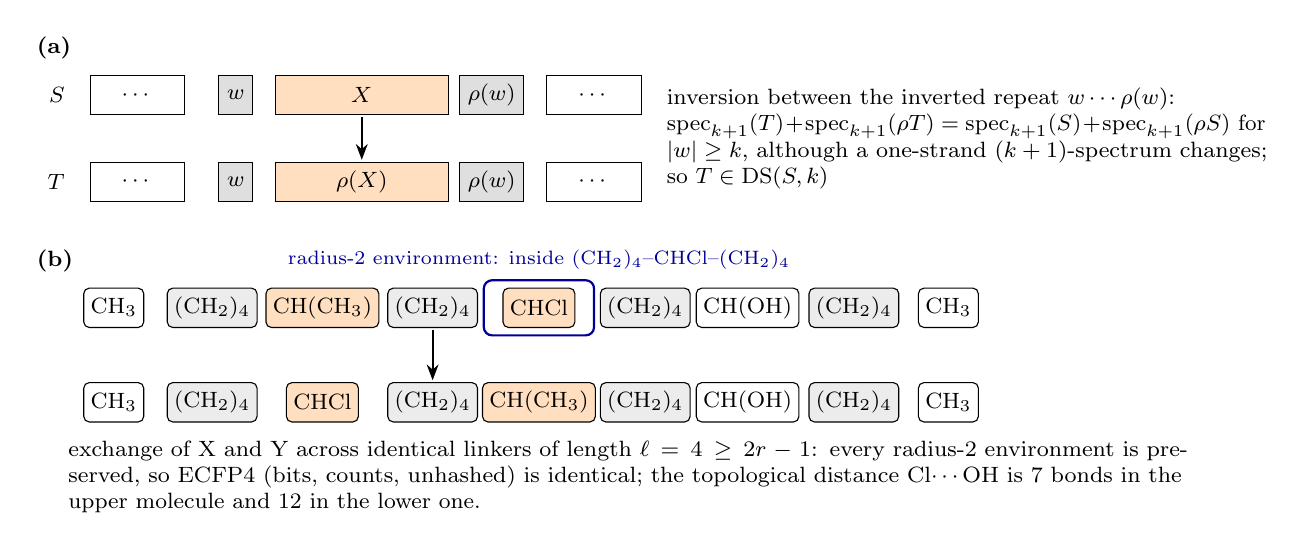
\begin{tikzpicture}[font=\small,
  seg/.style={draw, minimum height=0.5cm, inner sep=3pt, font=\footnotesize},
  rep/.style={seg, fill=gray!25},
  inv/.style={seg, fill=orange!25},
  atom/.style={draw, rounded corners=2pt, minimum height=0.5cm, inner sep=2.5pt, font=\footnotesize},
  lnk/.style={atom, fill=gray!15},
  lab/.style={font=\footnotesize, align=left, anchor=west}]
% ---------------- (a) inversion flip between an inverted repeat
\node[anchor=west, font=\bfseries\footnotesize] at (-0.6,3.6) {(a)};
\node[anchor=east, font=\footnotesize] at (0.0,3.0) {$S$};
\node[seg, minimum width=1.2cm] (a1) at (0.8,3.0) {$\cdots$};
\node[rep] (w1) at (2.05,3.0) {$w$};
\node[inv, minimum width=2.2cm] (x1) at (3.65,3.0) {$X$};
\node[rep] (rw1) at (5.3,3.0) {$\rho(w)$};
\node[seg, minimum width=1.2cm] (a2) at (6.6,3.0) {$\cdots$};
\node[anchor=east, font=\footnotesize] at (0.0,1.9) {$T$};
\node[seg, minimum width=1.2cm] at (0.8,1.9) {$\cdots$};
\node[rep] at (2.05,1.9) {$w$};
\node[inv, minimum width=2.2cm] at (3.65,1.9) {$\rho(X)$};
\node[rep] at (5.3,1.9) {$\rho(w)$};
\node[seg, minimum width=1.2cm] at (6.6,1.9) {$\cdots$};
\draw[-{Stealth[length=2mm]}, thick] (3.65,2.72) -- (3.65,2.18);
\node[lab, text width=7.6cm] at (7.4,2.45) {inversion between the inverted repeat $w\cdots\rho(w)$:
  $\spec_{k+1}(T)+\spec_{k+1}(\rho T)=\spec_{k+1}(S)+\spec_{k+1}(\rho S)$ for $|w|\ge k$, although a
  one-strand $(k+1)$-spectrum changes; so $T\in\DS(S,k)$};
% ---------------- (b) exchange across repeated linkers
\node[anchor=west, font=\bfseries\footnotesize] at (-0.6,0.9) {(b)};
\foreach \y/\X/\Y in {0.3/CH(CH$_3$)/CHCl, -0.9/CHCl/CH(CH$_3$)} {
  \node[atom] at (0.5,\y) {CH$_3$};
  \node[lnk] at (1.75,\y) {(CH$_2$)$_4$};
  \node[atom, fill=orange!25] at (3.15,\y) {\X};
  \node[lnk] at (4.55,\y) {(CH$_2$)$_4$};
  \node[atom, fill=orange!25] at (5.9,\y) {\Y};
  \node[lnk] at (7.25,\y) {(CH$_2$)$_4$};
  \node[atom] at (8.55,\y) {CH(OH)};
  \node[lnk] at (9.9,\y) {(CH$_2$)$_4$};
  \node[atom] at (11.1,\y) {CH$_3$};
}
\draw[-{Stealth[length=2mm]}, thick] (4.55,0.02) -- (4.55,-0.62);
% a radius-2 ball around the CHCl carbon of the first molecule
\draw[blue!60!black, thick, rounded corners=3pt] (5.2,-0.05) rectangle (6.6,0.65);
\node[font=\scriptsize, blue!60!black, anchor=south] at (5.9,0.66) {radius-2 environment: inside (CH$_2$)$_4$--CHCl--(CH$_2$)$_4$};
\node[lab, text width=14.6cm] at (-0.2,-1.85) {exchange of X and Y across identical linkers of length
  $\ell=4\ge2r-1$: every radius-2 environment is preserved, so ECFP4 (bits, counts, unhashed) is identical;
  the topological distance Cl$\cdots$OH is $7$ bonds in the upper molecule and $12$ in the lower one.};
\end{tikzpicture}}
\caption{Fibre-preserving moves under a symmetry. (a)~On double-stranded DNA, a segment $X$ flanked by an
inverted repeat $w\cdots\rho(w)$ may be replaced by its reverse complement. The double-stranded $(k+1)$-mer
spectrum is unchanged, so every strand-agnostic local encoder of order $k+1$ gives $S$ and $T$ the same output
\cite[Thm.~11.1]{AG}. (b)~The linker-$4$ pair of Table~\ref{tab:pairs}. Exchanging the two substituted carbons
across identical $(\mathrm{CH_2})_4$ linkers preserves every radius-$2$ atom environment; the two molecules are
distinct and place the chlorine and the hydroxyl at different distances.}\label{fig:moves}
\end{figure}

Table~\ref{tab:pairs} lists the pairs we checked, and Figure~\ref{fig:moves}b shows the first. The linker-$4$ pair,
\begin{center}\footnotesize
\texttt{CCCCCC(C)CCCCC(Cl)CCCCC(O)CCCCC}\quad and\quad\texttt{CCCCCC(Cl)CCCCC(C)CCCCC(O)CCCCC},
\end{center}
has identical ECFP4 in all three forms, and the two molecules place their pharmacophoric groups differently:
the shortest-path distance from the chlorine to the hydroxyl is $7$ bonds in the first and $12$ in the second,
while the methyl-to-chlorine distance is $7$ in both. A model that predicts a property from ECFP4 assigns the two
molecules the same value. Whether the property differs is a question about the property; the representation
cannot express the difference. A macrocycle with four substituents in two cyclic orders gives the same at
ECFP6 (Table~\ref{tab:pairs}). These examples are the exact analogue of the transposition move on sequences,
with the linker $u$ playing the role of the repeated $(k-1)$-mer.

\subsection{Stereochemistry}

The default Morgan fingerprint carries no stereochemistry. In RDKit, L- and D-alanine have identical ECFP4,
and so do (E)- and (Z)-2-butene; with the chirality option both pairs are separated. Enantiomers and
geometric isomers are thus fibres of the default fingerprint that a single flag removes. The collisions of
Table~\ref{tab:pairs} are not of this kind: no option of the algorithm separates them at the stated radius,
because the environments are identical as graphs.

% ================================================================ 5
\section{The unified quotient}\label{sec:unified}

The four settings share one structure. Let $\mathcal X$ be a set of objects (strings, circular strings, graphs),
let $G$ be a group acting on $\mathcal X$ (trivial, $\{e,\rho\}$, or the identity when the symmetry is already
inside the statistic), and let $\sigma_r\colon\mathcal X\to\mathcal M$ be a \emph{local statistic} of radius $r$, a
map to multisets of local pieces that is constant on $G$-orbits. The \emph{quotient map} is
$\pi=\sigma_r\colon\mathcal X\to\mathcal M$, and the \emph{fibre} of $x$ is $\Fib(x)=\pi^{-1}(\pi(x))$.

\begin{proposition}\label{prop:unified}
Let $\phi$ be any encoder that factors as $\phi=g\circ\sigma_r$. Then (i)~$\phi$ is $G$-invariant; (ii)~$\phi$ is
constant on $\Fib(x)$ for every $x$; (iii)~$\Fib(x)$ is a union of $G$-orbits and contains the orbit of $x$; and
(iv)~if $\sigma'_{r'}$ refines $\sigma_r$ (i.e.\ $\sigma_r=h\circ\sigma'_{r'}$), then the fibres of $\sigma'_{r'}$ are
contained in those of $\sigma_r$.
\end{proposition}

\begin{proof}
All four are immediate from the factorization and from the $G$-invariance of $\sigma_r$.
\end{proof}

\begin{table}[t]
\centering\small
\renewcommand{\arraystretch}{1.15}
\begin{tabular}{>{\raggedright\arraybackslash}p{0.2\textwidth}>{\raggedright\arraybackslash}p{0.15\textwidth}>{\raggedright\arraybackslash}p{0.24\textwidth}>{\raggedright\arraybackslash}p{0.30\textwidth}}
\toprule
encoder & objects, $G$ & local statistic $\sigma$ & fibre and its size\\
\midrule
composition, PseAAC ($\lambda\le k-1$), CNN of window $k$ with multiset pooling & strings, trivial & $k$-mer multiset (and first $(k-1)$-mer) & $F_k(S)$; one BEST determinant \cite{CC26a}\\
strand-agnostic DNA encoder of order $k+1$ & circular strings, $\{e,\rho\}$ & double-stranded $(k+1)$-mer multiset & $\DS(S,k)$; lattice sum of BEST determinants, $\#$P-hard \cite{AG}\\
ECFP$_{2r}$, Morgan count fingerprints & graphs, automorphisms of environments & multiset of radius-$r$ WL identifiers & on chains: symmetric coarsened window spectrum (Thm.~\ref{thm:chain}); in general the WL-$r$ class\\
\bottomrule
\end{tabular}
\caption{The quotient framework across the four encoder families.}\label{tab:unified}
\end{table}

Table~\ref{tab:unified} instantiates the framework. What differs between the rows is how hard the fibre is to
count and how large it is. On one strand the fibre is a determinant. With a free involution on the arcs it
becomes a lattice sum whose evaluation is $\#$P-hard. On graphs the fibre is the class of the $r$-round
Weisfeiler--Lehman refinement, whose enumeration is not known to be tractable at all, but whose members can be
constructed by the transposition principle wherever the graph contains repeated linkers. The framework also
says what the escapes are, in every row alike: an encoder leaves the fibre only by using a statistic that is not
a function of $\sigma_r$, e.g.\ a larger radius, absolute position, or, for molecules, three-dimensional
coordinates or stereo flags.

% ================================================================ 6
\section{Discussion}\label{sec:discussion}

Symmetry makes fibres larger and harder to count, but it does not change their nature. In both settings the
fibre is generated by moves that exchange interchangeable pieces across repeated boundaries: segments between
repeated $k$-mers on one strand, additionally segments between inverted repeats on two strands, and blocks
between repeated linkers in a molecular graph. In each case the move preserves the local content exactly, and in
each case it changes something a downstream task may depend on: the gene order of a genome, or the distance
between two pharmacophores.

Two limitations. The exact description of Morgan fibres (Theorem~\ref{thm:chain}) is for substituted chains; for
general graphs we have only the WL characterization and explicit constructions. And we did not measure any
molecular property on the collision pairs: whether the linker-$4$ pair differs in a bioassay is an experimental
question. What is settled is that no model reading ECFP4 can predict such a difference.

\section*{Data and code availability}
\sloppy
\texttt{code/ecfp\_fibres.py} (Python, RDKit 2026.03.6) reproduces Section~\ref{sec:ecfp}: the collision pairs and
their fingerprints at radii $1$--$4$, the pharmacophore distances, the exhaustive check of
Theorem~\ref{thm:chain} for $N=9$ and the census, and the stereochemical examples; its transcript is
\texttt{results/ecfp\_fibres\_output.txt}. The $\phi$X174 numbers of Section~\ref{sec:phix} are those of the
verification scripts of the monograph's repository (\texttt{ds\_lattice.py}, \texttt{ds\_flips.py},
\texttt{ds\_fermion.py}, \texttt{ds\_count.py} at \url{https://github.com/Ruqing1963/algebraic-genomics}), whose
transcripts we quote. The genome (NC\_001422.1) is included. Code, data and this paper are at
\url{https://github.com/Ruqing1963/symmetry-fibres} and are archived at \doi{10.5281/zenodo.23002923}.

\section*{Funding}
This project was supported by the National Natural Science Foundation of China (No.~22464010), the
Guangxi Natural Science Foundation of China (No.~2025GXNSFAA069294), and the 2025 Bagui Youth Top
Talent Project.

\begin{thebibliography}{99}
\bibitem{BEST} T.~van Aardenne-Ehrenfest, N.~G.~de Bruijn, \emph{Circuits and trees in oriented linear
graphs}, Simon Stevin \textbf{28} (1951) 203--217.
\bibitem{AG} R.~Chen, \emph{Algebraic Genomics: The Combinatorics of Sequence Reconstruction and
Representation}, monograph, Zenodo (2026). \doi{10.5281/zenodo.22943487}
\bibitem{CC26a} Z.~Chen, R.~Chen, \emph{What a local encoder cannot see: spectral fibres of the human proteome
and the representation of perturbagens}, Zenodo (2026). \doi{10.5281/zenodo.22950095}
\bibitem{CC26b} Z.~Chen, R.~Chen, \emph{Separation without resolution: the spectral fibre geometry of the human
proteome and the blind spots of local sequence encoders}, Zenodo (2026). \doi{10.5281/zenodo.22959211}
\bibitem{CC26c} Z.~Chen, R.~Chen, \emph{Information loss and quotient geometry of local sequence encoders:
representation lattices, fibre entropy and diameter bounds}, Zenodo (2026). \doi{10.5281/zenodo.22960439}
\bibitem{CC26d} Z.~Chen, R.~Chen, \emph{What finite-receptive-field encoders cannot distinguish: invariance
theorems and architectural boundaries of convolutional sequence models}, Zenodo (2026).
\doi{10.5281/zenodo.22963882}
\bibitem{CC26e} Z.~Chen, R.~Chen, \emph{Biologically reachable spectral fibres: repeat shuffling, copy
ambiguity and the scarcity of cryptic pathogenic missense variants in ClinVar}, Zenodo (2026).
\doi{10.5281/zenodo.22966020}
\bibitem{RDKit} G.~Landrum et al., \emph{RDKit: open-source cheminformatics}, version 2026.03.6,
\url{https://www.rdkit.org}.
\bibitem{Morgan65} H.~L.~Morgan, \emph{The generation of a unique machine description for chemical
structures: a technique developed at Chemical Abstracts Service}, J.\ Chem.\ Doc.\ \textbf{5} (1965) 107--113.
\doi{10.1021/c160017a018}
\bibitem{Pev95} P.~A.~Pevzner, \emph{DNA physical mapping and alternating Eulerian cycles in colored
graphs}, Algorithmica \textbf{13} (1995) 77--105. \doi{10.1007/bf01188582}
\bibitem{RH10} D.~Rogers, M.~Hahn, \emph{Extended-connectivity fingerprints}, J.\ Chem.\ Inf.\ Model.\
\textbf{50} (2010) 742--754. \doi{10.1021/ci100050t}
\bibitem{Ukk92} E.~Ukkonen, \emph{Approximate string-matching with $q$-grams and maximal matches},
Theoret.\ Comput.\ Sci.\ \textbf{92} (1992) 191--211. \doi{10.1016/0304-3975(92)90143-4}
\bibitem{WL68} B.~Weisfeiler, A.~Leman, \emph{The reduction of a graph to canonical form and the algebra which
appears therein}, Nauchno-Technicheskaya Informatsia, Ser.~2, \textbf{9} (1968) 12--16.
\bibitem{GIN} K.~Xu, W.~Hu, J.~Leskovec, S.~Jegelka, \emph{How powerful are graph neural networks?},
International Conference on Learning Representations (2019).
\end{thebibliography}

\end{document}
